%% LyX 2.1.3 created this file.  For more info, see http://www.lyx.org/.
%% Do not edit unless you really know what you are doing.
\documentclass{article} 
\usepackage{ucs}
\usepackage[utf8x]{inputenc}
\usepackage[sc]{mathpazo}
\usepackage[T1]{fontenc}
\usepackage{geometry}

\newenvironment{uzdevums}[1][\unskip]{%
\vspace{3mm}
\noindent
\textbf{#1 uzdevums:}
\noindent}
{}

\geometry{verbose,tmargin=2.5cm,bmargin=2.5cm,lmargin=2.5cm,rmargin=2.5cm}
\setcounter{secnumdepth}{2}
\setcounter{tocdepth}{2}
\usepackage{url}
\usepackage[unicode=true,pdfusetitle,
 bookmarks=true,bookmarksnumbered=true,bookmarksopen=true,bookmarksopenlevel=2,
 breaklinks=false,pdfborder={0 0 1},backref=false,colorlinks=false]
 {hyperref}
\renewcommand{\abstractname}{Anotācija}
\hypersetup{
 pdfstartview={XYZ null null 1}}
\begin{document}





\title{42.\ AMO rezultāti tabulās un zīmējumos}

\author{}
\date{}

\maketitle

\begin{abstract}
Šajā dokumentā apkopoti daži 42.\ Atklātās matemātikas olimpiādes (2015.m.g.) rezultātu kop\-sa\-vil\-ku\-mi. Izmantojot izklājlapas, ko publisko LU Neklātienes Matemātikas Skola, aprēķināts dalībnieku skaits, dalības aktivitāte (AMO dalībnieku īpatsvars no visiem attiecīgā vecuma skolēniem), dalība un rezultāti atkarībā no skolēnu \v{g}eogrāfijas, urbanizācijas, valodas, dzimuma. Apkopoti saraksti ar skolotājiem un skolām, kas nodrošinājuši augstu dalību vai ieguvuši lielu punktu kopskaitu. Pārskata nobeigumā minēti dati arī par uzdevumiem --- vidējais punktu skaits un vērtējumu sadalījums, kāda daļa no rēķinātājiem neuzsāka risināt (``mīnusu'' jeb neatrasto risinājumu skaits galavērtējumā), kāda ir konkrētā uzdevuma vērtējumu korelācija ar pārējo uzdevumu vērtējumu summu. 
\end{abstract}

\section{Dalībnieku aktivitāte}

Šajā sadaļā atbildēsim uz jautājumu, kāda daļa no katrai klasei atbilstošās vecuma grupas skolēniem piedalījās 42.\ AMO. 
Dati par skolēnu skaitu pa re\v{g}ioniem, klasēm un mācību valodām ņemti no IZM publiskotās statistikas --- \url{http://izm.gov.lv/lv/publikacijas-un-statistika/statistika-par-visparejo-izglitibu/2014-2015-m-g}. Dati apkopoti par 9 lielajām pilsētām kā arī par re\v{g}ioniem, kuros nav ietvertas lielās pilsētas. Ar {\em re\v{g}ioniem} domāti NUTS 3 re\v{g}ioni --- sk. \url{http://en.wikipedia.org/wiki/Statistical_regions_of_Latvia} - Kurzeme, Latgale, Pierīga Rīga, Vidzeme, Zemgale.


\subsection{Dalība olimpiādē}

\begin{knitrout}
\definecolor{shadecolor}{rgb}{0.969, 0.969, 0.969}\color{fgcolor}\begin{kframe}


{\ttfamily\noindent\bfseries\color{errorcolor}{\#\# Error in setwd("{}/home/st/ddgatve-stat/reports/"{}): cannot change working directory}}

{\ttfamily\noindent\bfseries\color{errorcolor}{\#\# Error in eval(expr, envir, enclos): could not find function "{}getExtResults"{}}}

{\ttfamily\noindent\bfseries\color{errorcolor}{\#\# Error in nrow(results): object 'results' not found}}\end{kframe}
\end{knitrout}

%% col1 = region
%% col2 = participants
%% col3 = total guys
%% col4 = percentage participated

\begin{knitrout}
\definecolor{shadecolor}{rgb}{0.969, 0.969, 0.969}\color{fgcolor}\begin{kframe}


{\ttfamily\noindent\bfseries\color{errorcolor}{\#\# Error in table(results\$Region14): object 'results' not found}}

{\ttfamily\noindent\bfseries\color{errorcolor}{\#\# Error in FUN(X[[i]], ...): object 'ttParticipants' not found}}

{\ttfamily\noindent\bfseries\color{errorcolor}{\#\# Error in eval(expr, envir, enclos): object 'activityParticipants' not found}}

{\ttfamily\noindent\bfseries\color{errorcolor}{\#\# Error in eval(expr, envir, enclos): could not find function "{}getAllPupils"{}}}

{\ttfamily\noindent\bfseries\color{errorcolor}{\#\# Error in FUN(X[[i]], ...): object 'allPupils' not found}}

{\ttfamily\noindent\bfseries\color{errorcolor}{\#\# Error in eval(expr, envir, enclos): object 'activityAllPupils' not found}}

{\ttfamily\noindent\bfseries\color{errorcolor}{\#\# Error in matrix(c(activityParticipants, activityAllPupils, 100 * activityParticipants/activityAllPupils), : object 'activityParticipants' not found}}

{\ttfamily\noindent\bfseries\color{errorcolor}{\#\# Error in eval(expr, envir, enclos): object 'activityParticipants' not found}}

{\ttfamily\noindent\bfseries\color{errorcolor}{\#\# Error in inherits(x, "{}list"{}): object 'activityTable' not found}}\end{kframe}
\end{knitrout}



\begin{knitrout}
\definecolor{shadecolor}{rgb}{0.969, 0.969, 0.969}\color{fgcolor}\begin{kframe}


{\ttfamily\noindent\bfseries\color{errorcolor}{\#\# Error in rev((100 * activityParticipants/activityAllPupils)[1:14]): object 'activityParticipants' not found}}

{\ttfamily\noindent\bfseries\color{errorcolor}{\#\# Error in barplot(aa, names.arg = bb, horiz = TRUE, las = 1, main = "{}Number of Participants per Region (\%)"{}): object 'aa' not found}}

{\ttfamily\noindent\bfseries\color{errorcolor}{\#\# Error in int\_abline(a = a, b = b, h = h, v = v, untf = untf, ...): plot.new has not been called yet}}

{\ttfamily\noindent\bfseries\color{errorcolor}{\#\# Error in int\_abline(a = a, b = b, h = h, v = v, untf = untf, ...): object 'meanActivity' not found}}\end{kframe}
\end{knitrout}


Ir svarīgs ne tikai dalībnieku skaits, bet arī viņu sagatavotības līmenis. Šajā grafikā ikviena olimpiādes dalībnieka rezultātam ir aprēķināta z-normalizētā vērtība jeb {\em z-score}, t.i. no iegūtā punktu skaita jeb {\em raw score} atņem attiecīgās klases aritmētisko vidējo un izdala ar attiecīgās klases standartnovirzi. Pēc tam katrā re\v{g}ionā un katrā klašu grupā atsevišķi rēķina šo z-normalizēto vērtību aritmētisko vidējo. Kā redzams diagrammā, vislabākie vērtējumi olimpiādēs ir Rīgā (sarkanais grafiks) un Latgalē (zilais grafiks).


\begin{knitrout}
\definecolor{shadecolor}{rgb}{0.969, 0.969, 0.969}\color{fgcolor}\begin{kframe}


{\ttfamily\noindent\bfseries\color{errorcolor}{\#\# Error in mean(results\$Summa[results\$Grade == gg]): object 'results' not found}}

{\ttfamily\noindent\bfseries\color{errorcolor}{\#\# Error in is.data.frame(x): object 'results' not found}}

{\ttfamily\noindent\bfseries\color{errorcolor}{\#\# Error in mean(results\$Summa[results\$Region6 == actRegion \& results\$Grade == : object 'results' not found}}

{\ttfamily\noindent\color{warningcolor}{\#\# Warning in min(x): no non-missing arguments to min; returning Inf}}

{\ttfamily\noindent\color{warningcolor}{\#\# Warning in max(x): no non-missing arguments to max; returning -Inf}}

{\ttfamily\noindent\color{warningcolor}{\#\# Warning in min(x): no non-missing arguments to min; returning Inf}}

{\ttfamily\noindent\color{warningcolor}{\#\# Warning in max(x): no non-missing arguments to max; returning -Inf}}

{\ttfamily\noindent\bfseries\color{errorcolor}{\#\# Error in plot.window(...): need finite 'ylim' values}}

{\ttfamily\noindent\bfseries\color{errorcolor}{\#\# Error in gradesMatrix[, i]: subscript out of bounds}}\end{kframe}

{\centering 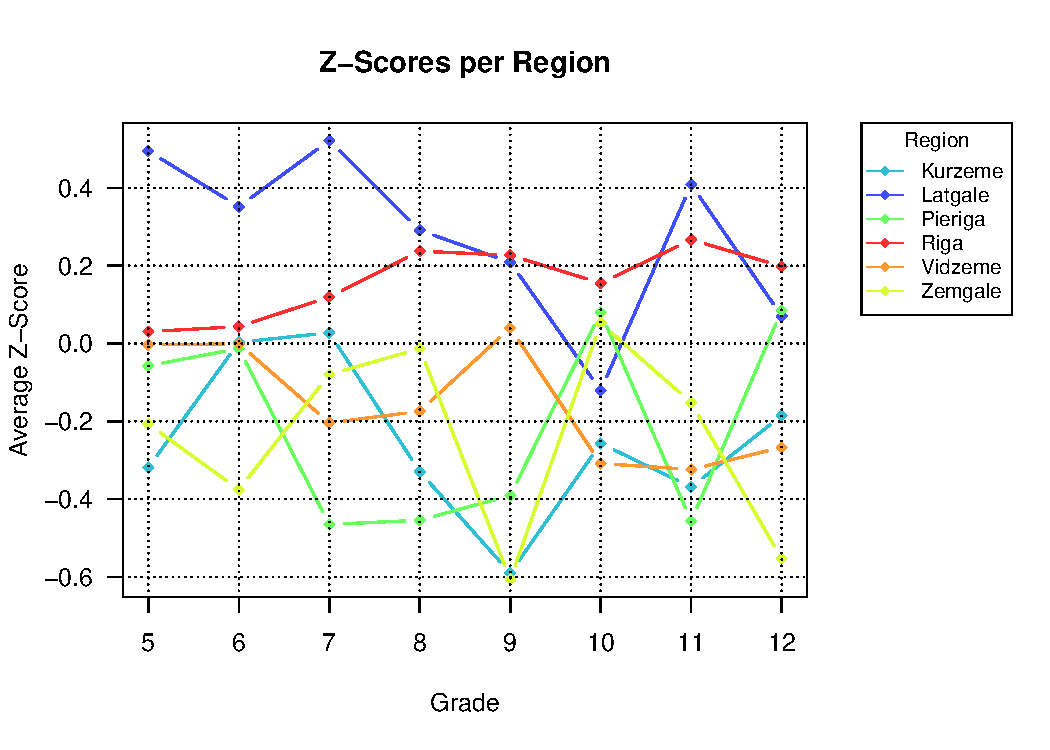
\includegraphics[width=\maxwidth]{figure/minimal-averages-per-region-1} 

}



\end{knitrout}



% 1+9+5 aktivitāšu skaitļi pa reģioniem
% Katram no 15 reģioniem dota dzimumu proporcija
%% Stabiņi grupās pa 3 - visi/meitenes/zēni. 

% 1+9+5 aktivitāšu skaitļi pa reģioniem - darbi latviešu valodā
% Katram no 15 reģioniem dota dzimumu proporcija

% 1+9+5 aktivitāšu skaitļi pa reģioniem - darbi krievu valodā
% Katram no 15 reģioniem dota dzimumu proporcija

\begin{knitrout}
\definecolor{shadecolor}{rgb}{0.969, 0.969, 0.969}\color{fgcolor}\begin{kframe}


{\ttfamily\noindent\bfseries\color{errorcolor}{\#\# Error in table(results\$Grade): object 'results' not found}}

{\ttfamily\noindent\bfseries\color{errorcolor}{\#\# Error in pie(pieVals, labels = paste0("{}Grade "{}, 5:12, "{} ("{}, pieVals, "{})"{}), : object 'pieVals' not found}}\end{kframe}
\end{knitrout}

\subsection{Dalība un sociāli-ekonomiskie rādītāji}

% Trīs 14-bumbulīšu diagrammas

Šeit varētu ievietot diagrammas pa novadiem vai novadu grupām, kas parāda divu parametru attiecību (varētu būt runa par burbulīšu diagrammām, ko zīmē divās dimensijās; turklāt burbulīša laukums ir aptuveni proporcionāls skolēnu skaitam olimpiādē).

\begin{itemize}
\item Sociāli-ekonomisko rādītāju --- bezdarbu, IIN uz 1 iedzīvotāju, pašvaldības izdevumus uz 1 skolēnu vai skolēnu skaitu skolā.
\item Dalībnieku aktivitāti (dalībnieku attiecību pret visiem skolēniem novadā) kā arī olimpiādes summāro rezultātu (punktu summas attiecību pret visiem skolēniem novadā). 
\end{itemize}

Šādas diagrammas palīdzētu saprast, kādi sociālie priekšnoteikumi veicina interesi par olimpiādēm, kāda izglītības politika (piemēram, mazo skolu saglabāšana vai slēgšana; lielāki vai mazāki izdevumi par vienu skolēnu) varētu pozitīvi iespaidot olimpiāžu rezultātus. 

\subsection{Dalībnieku struktūra}



%% Segmenti -- 6 NUTS reģioni
% http://en.wikipedia.org/wiki/Statistical_regions_of_Latvia

Atklātajā matemātikas olimpiādē sastopami darbi latviešu un krievu valodās. Valodu būtu visprecīzāk noteikt, aplūkojot katru konkrēto darbu.Katras klases joslas iekšpusē iezīmēts balts aplītis, kurš parāda latviešu skolēnu īpatsvaru visu attiecīgās klases audzēkņu vidū. Izņemot 5.\ un 6.\ klasi, latviešu darbu īpatsvars 42.\ AMO ir nedaudz lielāks nekā skolēnu īpatsvars latviešu plūsmas skolās kopumā. Latvijas vispārizglītojošajās skolās mācības mēdz notikt arī poļu, ukraiņu, baltkrievu, angļu un franču valodās. Šo skolu audzēkņi var izvēlēties rakstīt darbu latviski vai krieviski. Viņu darbi pieskaitīti atkarībā no re\v{g}istrācijā norādītās valodas.


%% K/L skaita attiecība pa klasēm 
\begin{knitrout}
\definecolor{shadecolor}{rgb}{0.969, 0.969, 0.969}\color{fgcolor}\begin{kframe}


{\ttfamily\noindent\bfseries\color{errorcolor}{\#\# Error in table(results\$Grade, results\$Language): object 'results' not found}}

{\ttfamily\noindent\bfseries\color{errorcolor}{\#\# Error in matrix(c(langtab[, "{}L"{}]/rowSums(langtab), langtab[, "{}K"{}]/rowSums(langtab)), : object 'langtab' not found}}

{\ttfamily\noindent\bfseries\color{errorcolor}{\#\# Error in barplot(langmat/colSums(langmat), las = 1, col = c("{}darkgreen"{}, : object 'langmat' not found}}

{\ttfamily\noindent\bfseries\color{errorcolor}{\#\# Error in plot.xy(xy.coords(x, y), type = type, ...): plot.new has not been called yet}}\end{kframe}
\end{knitrout}



%% Marimekko diagrammas - dalībnieku dzimumu struktūra pa reģioniem. 
% https://learnr.wordpress.com/2009/03/29/ggplot2_marimekko_mosaic_chart/
%% Segmenti -- 4 urbanizācijas tipi (LV-meitenes, LV-zēni, RU-meitenes, RU-zēni)

Dalībnieku demogrāfisko struktūru var attēlot arī dažādām parametru kombinācijām. Šajā zīmējumā redzams dalībnieku sadalījums pa klasēm (vertikālie stabiņi), un katras klases iekšienē --- arī pa darbu valodām un dalībnieku dzimumiem. Skolēna dzimums re\v{g}istrācijas un rezultātu datos nav dots, 42.\ AMO tos noteicām pēc skolēna vārda. Pasaulē ir matemātikas sacensības, piemēram, EGMO (European Girls' Mathematical Olympiad), kuru nolūks ir veicināt meiteņu pievēršanos eksaktajām un inženierzinātnēm. Kopš olimpiādes pirmsākumiem (2012.\ gadā Kembridžā) EGMO piedalās arī četras vecāko klašu skolnieces no Latvijas. Sk. \url{https://www.egmo.org/}.

Latviešu valodā rakstītajiem darbiem zēnu un meiteņu ir aptuveni vienāds skaits, bet krievu valodā rakstītajiem darbiem meiteņu vecāko klašu grupās ir ievērojami mazāk nekā zēnu.


\begin{knitrout}
\definecolor{shadecolor}{rgb}{0.969, 0.969, 0.969}\color{fgcolor}\begin{kframe}


{\ttfamily\noindent\bfseries\color{errorcolor}{\#\# Error in library(reshape): there is no package called 'reshape'}}

{\ttfamily\noindent\bfseries\color{errorcolor}{\#\# Error in eval(expr, envir, enclos): could not find function "{}getExtResults"{}}}

{\ttfamily\noindent\bfseries\color{errorcolor}{\#\# Error in table(results\$Grade): object 'results' not found}}

{\ttfamily\noindent\bfseries\color{errorcolor}{\#\# Error in eval(expr, envir, enclos): object 'pupilsPerGrade' not found}}

{\ttfamily\noindent\bfseries\color{errorcolor}{\#\# Error in table(results\$Grade[results\$Dzimums == "{}Male"{} \& results\$Language == : object 'results' not found}}

{\ttfamily\noindent\bfseries\color{errorcolor}{\#\# Error in table(results\$Grade[results\$Dzimums == "{}Female"{} \& results\$Language == : object 'results' not found}}

{\ttfamily\noindent\bfseries\color{errorcolor}{\#\# Error in table(results\$Grade[results\$Dzimums == "{}Male"{} \& results\$Language == : object 'results' not found}}

{\ttfamily\noindent\bfseries\color{errorcolor}{\#\# Error in table(results\$Grade[results\$Dzimums == "{}Female"{} \& results\$Language == : object 'results' not found}}

{\ttfamily\noindent\bfseries\color{errorcolor}{\#\# Error in data.frame(segment = 5:12, segpct = pupilsPerGradePercent, lv.males = AlphaVals, : object 'pupilsPerGradePercent' not found}}

{\ttfamily\noindent\bfseries\color{errorcolor}{\#\# Error in df\$segpct: object of type 'closure' is not subsettable}}

{\ttfamily\noindent\bfseries\color{errorcolor}{\#\# Error in df\$xmax: object of type 'closure' is not subsettable}}

{\ttfamily\noindent\bfseries\color{errorcolor}{\#\# Error in df\$segpct <- NULL: object of type 'closure' is not subsettable}}

{\ttfamily\noindent\bfseries\color{errorcolor}{\#\# Error in eval(expr, envir, enclos): could not find function "{}melt"{}}}

{\ttfamily\noindent\bfseries\color{errorcolor}{\#\# Error in empty(.data): object 'dfm' not found}}

{\ttfamily\noindent\bfseries\color{errorcolor}{\#\# Error in empty(.data): object 'dfm1' not found}}

{\ttfamily\noindent\bfseries\color{errorcolor}{\#\# Error in with(dfm1, xmin + (xmax - xmin)/2): object 'dfm1' not found}}

{\ttfamily\noindent\bfseries\color{errorcolor}{\#\# Error in with(dfm1, ymin + (ymax - ymin)/2): object 'dfm1' not found}}

{\ttfamily\noindent\bfseries\color{errorcolor}{\#\# Error in ggplot(dfm1, aes(ymin = ymin, ymax = ymax, xmin = xmin, xmax = xmax, : object 'dfm1' not found}}

{\ttfamily\noindent\bfseries\color{errorcolor}{\#\# Error in eval(expr, envir, enclos): object 'p' not found}}

{\ttfamily\noindent\bfseries\color{errorcolor}{\#\# Error in eval(expr, envir, enclos): object 'p1' not found}}

{\ttfamily\noindent\bfseries\color{errorcolor}{\#\# Error in eval(expr, envir, enclos): object 'p2' not found}}

{\ttfamily\noindent\bfseries\color{errorcolor}{\#\# Error in eval(expr, envir, enclos): object 'p3' not found}}\end{kframe}
\end{knitrout}

\subsection{Dalībnieku valodas lielajās pilsētās}

Šajā diagrammā mazie aplīši parāda olimpiādes darbu valodu proporciju Latvijas lielākajās pilsētās (9 lielās pilsētas kā arī Ogre, Tukums un Cēsis, kurās iedzīvotāju skaits ir tuvu 20 tūkstošiem - t.i. daudz neatšķiras no Valmieras un Jēkabpils iedzīvotāju skaita). Aplīša laukums ir aptuveni proporcionāls dalībnieku skaitam no attiecīgās pilsētas.

\begin{knitrout}
\definecolor{shadecolor}{rgb}{0.969, 0.969, 0.969}\color{fgcolor}\begin{kframe}


{\ttfamily\noindent\bfseries\color{errorcolor}{\#\# Error in table(results\$Municipality): object 'results' not found}}

{\ttfamily\noindent\bfseries\color{errorcolor}{\#\# Error in table(results\$Municipality[results\$Language == "{}L"{}]): object 'results' not found}}

{\ttfamily\noindent\bfseries\color{errorcolor}{\#\# Error in table(results\$Municipality[results\$Language == "{}K"{}]): object 'results' not found}}

{\ttfamily\noindent\bfseries\color{errorcolor}{\#\# Error in langLV[is.na(langLV)] <- 0: object 'langLV' not found}}

{\ttfamily\noindent\bfseries\color{errorcolor}{\#\# Error in langRU[is.na(langRU)] <- 0: object 'langRU' not found}}

{\ttfamily\noindent\bfseries\color{errorcolor}{\#\# Error in eval(expr, envir, enclos): object 'langAll' not found}}

{\ttfamily\noindent\bfseries\color{errorcolor}{\#\# Error in eval(expr, envir, enclos): object 'totals' not found}}

{\ttfamily\noindent\bfseries\color{errorcolor}{\#\# Error in is.unit(width): object 'sizemult' not found}}\end{kframe}

{\centering 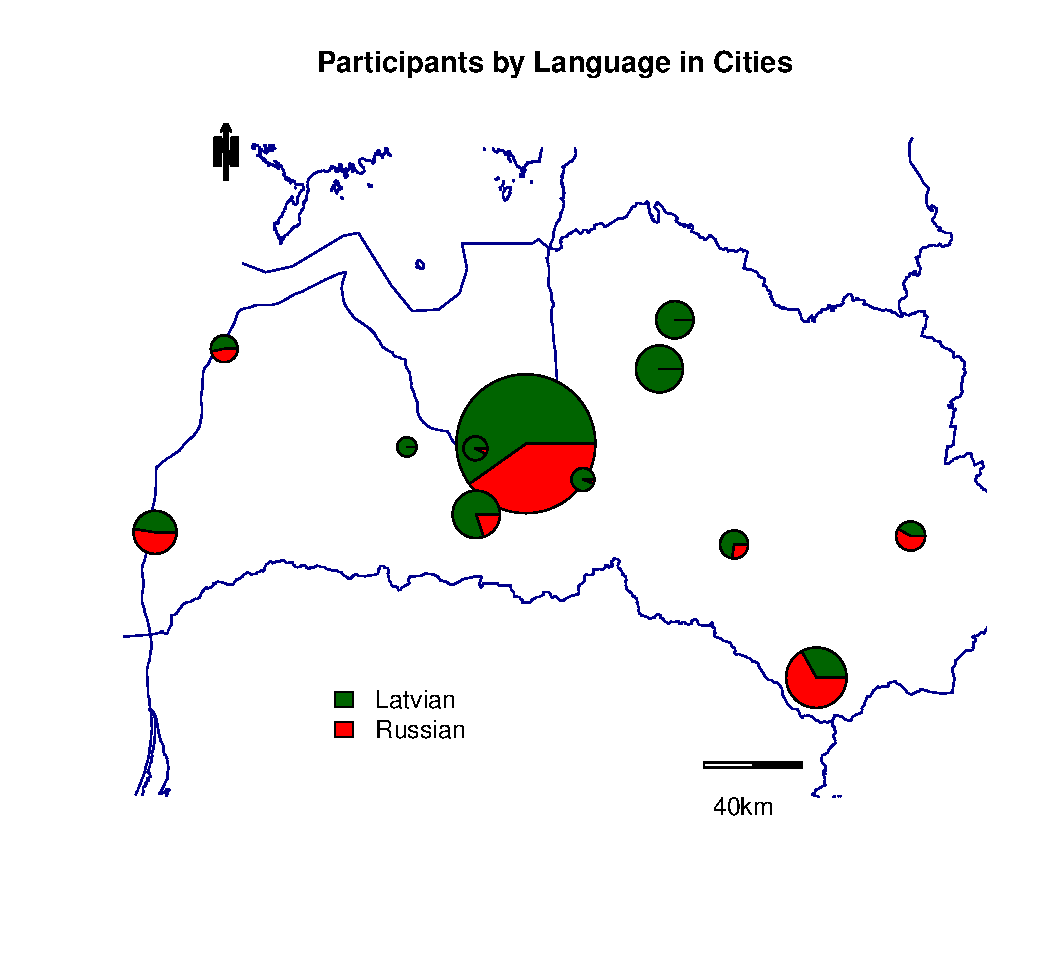
\includegraphics[width=\maxwidth]{figure/minimal-language-per-city-1} 

}



\end{knitrout}





\section{Vidējie rezultāti dalībnieku kategorijām}

Zīmējumā dots rezultātu intervāls katrai klasei. ``Kastītes'' kreisā mala atbilst apakšējai kvartilei, labā mala --- augšējai kvartilei, bet platā zilā svītriņa vidū --- mediānai. Ja klases darbus sakārtotu punktu pieaugšanas secībā un sadalītu četrās vienādās daļās, tad viszemāko punktu ieguvēju ceturtdaļa atrastos uz kreisās ūsas, divas vidējās ceturtdaļas --- kastītes iekšpusē, bet augšējā ceturtdaļa --- uz labās ūsas. Šī diagramma parāda, ka atkarībā no klašu grupas, var  atšķirties punktu skaits, kas nepieciešams nonākšanai līdz ``vidusmēram'' vai līdz augšējai ceturtdaļai. 

\begin{knitrout}
\definecolor{shadecolor}{rgb}{0.969, 0.969, 0.969}\color{fgcolor}\begin{kframe}


{\ttfamily\noindent\bfseries\color{errorcolor}{\#\# Error in eval(expr, envir, enclos): object 'results' not found}}

{\ttfamily\noindent\bfseries\color{errorcolor}{\#\# Error in int\_abline(a = a, b = b, h = h, v = v, untf = untf, ...): plot.new has not been called yet}}\end{kframe}
\end{knitrout}




%% Visu dalībnieku darbi, iekrāsotas godalgotās vietas 
%% Meiteņu un zēnu darbi (Meitenes zīmējam tanī pašā histogrammā)
%% Meitenes ir sazīmētas apakšā. 

%% Urbaniz. tips. Rīgas, 8 lielo pilsētu, mazpilsētu un lauku darbi

%% Latviešu un krievu valodā rakstītie darbi

%% Latviešu un krievu valodā rakstītie darbi -- tikai 9 lielajās pilsētās


\section{Skolas un skolotāji}

\begin{knitrout}
\definecolor{shadecolor}{rgb}{0.969, 0.969, 0.969}\color{fgcolor}\begin{kframe}


{\ttfamily\noindent\bfseries\color{errorcolor}{\#\# Error in eval(expr, envir, enclos): could not find function "{}getUpperQuartiles"{}}}

{\ttfamily\noindent\bfseries\color{errorcolor}{\#\# Error in paste0("{}\$Q\_3(Grade"{}, 5:12, "{})="{}, upQuartiles, "{}\textbackslash{}\textbackslash{};\$"{}): object 'upQuartiles' not found}}

{\ttfamily\noindent\bfseries\color{errorcolor}{\#\# Error in paste(quartileStr, sep = "{}; "{}): object 'quartileStr' not found}}\end{kframe}
\end{knitrout}





































